\documentclass[11pt]{article}
\usepackage[margin=0.8in]{geometry}
\usepackage{amsmath,amssymb,hyperref,booktabs,graphicx}
\title{Symbolic signed-graph reduction for pencil relations}
\author{Mathematical implementation and development checks}
\date{28 October 2026 (America/Los\_Angeles)}
\begin{document}\maketitle
\noindent The existing pencil cohort has 543 verified candidate targets out of
1,260. This packet adds a native algebraic component, with no new cohort or
performance measurement. Its candidate/rho cost ratio is unknown.
\section*{Algebraic interface}
An input row is $\sum a_iX_i+\sum b_jS_j=0$ over a prime field. At most two
large-variable terms survive canonicalization; the $S_j$ remain symbolic.
The forest stores $X_i=s_iX_{\mathrm{parent}(i)}+u_i(S)$ and uses union by size.
Root substitution leaves zero, one or two free roots. Zero emits a constraint,
one anchors a root, and two join components by an invertible pivot.
An unbalanced signed cycle anchors its root; it does not immediately yield
an additional relation involving only small variables.
\section*{Recorded development checks}
The Rust suite compares the emitted small-row space with independent dense
row reduction after every prefix: 40 prefixes, 128 deterministic streams and
five prime fields (2, 3, 5, 7 and 101), totaling 25,600 checks.
Additional cases cover signed cycles, duplicate terms, rejected inputs,
composites and a prime near the 64-bit limit. The test log is retained.
The four Lean declarations cover pivot equivalence, substitution, balanced
cycles and unbalanced cycles. Their direct compiler result and axiom report
are retained separately. They do not formalize the full forest invariant or
prove correspondence with Rust.
The retained residual basis is now also compared with the independent reference
at all 25,600 prefixes. Seven native tests pass. Explicit working and retained
coefficient caps leave the basis unchanged on rejection; callers must stop or
retain that rejected row. Logical counters include failed attempts but omit
map comparisons, allocation, setup and exponentiation internals. These are
coefficient limits, not process-memory guarantees or a complete cost model.
\section*{Next integration gates}
\begin{tabular}{p{0.61\linewidth}p{0.28\linewidth}}\toprule
Requirement & Status\\\midrule
Prime-field row kernel and independent prefix tests & Implemented and tested\\
Forest-state induction and Rust correspondence & Open\\
Pencil adapter, fixed small-base selection and admission accounting & Open\\
Full symbolic-vector, memory and residual elimination costs & Unmeasured\\
Remaining 717 frozen candidate targets & No new results\\
End-to-end cost against matched rho & Unknown\\\bottomrule
\end{tabular}
\section*{Sources and limitations}
The graph construction follows the mathematical distinction between full
relations and cycles leaving a large prime in Gaudry, Theriault and Thome,
\href{https://cacr.uwaterloo.ca/techreports/2004/corr2004-29.pdf}{double large prime
variation}, sections 2.3 and 3.1 (2005 version). Its genus-at-least-three
complexity result is not asserted for this genus-2 pencil stream. Existing
repository graph and large-prime eliminators informed the implementation.
The editable graph is \texttt{reduction.svg}; the machine-readable check
table is \texttt{checks.csv}. All results are development checks; no runtime,
memory improvement or full-cohort completion is inferred from them.
\begin{center}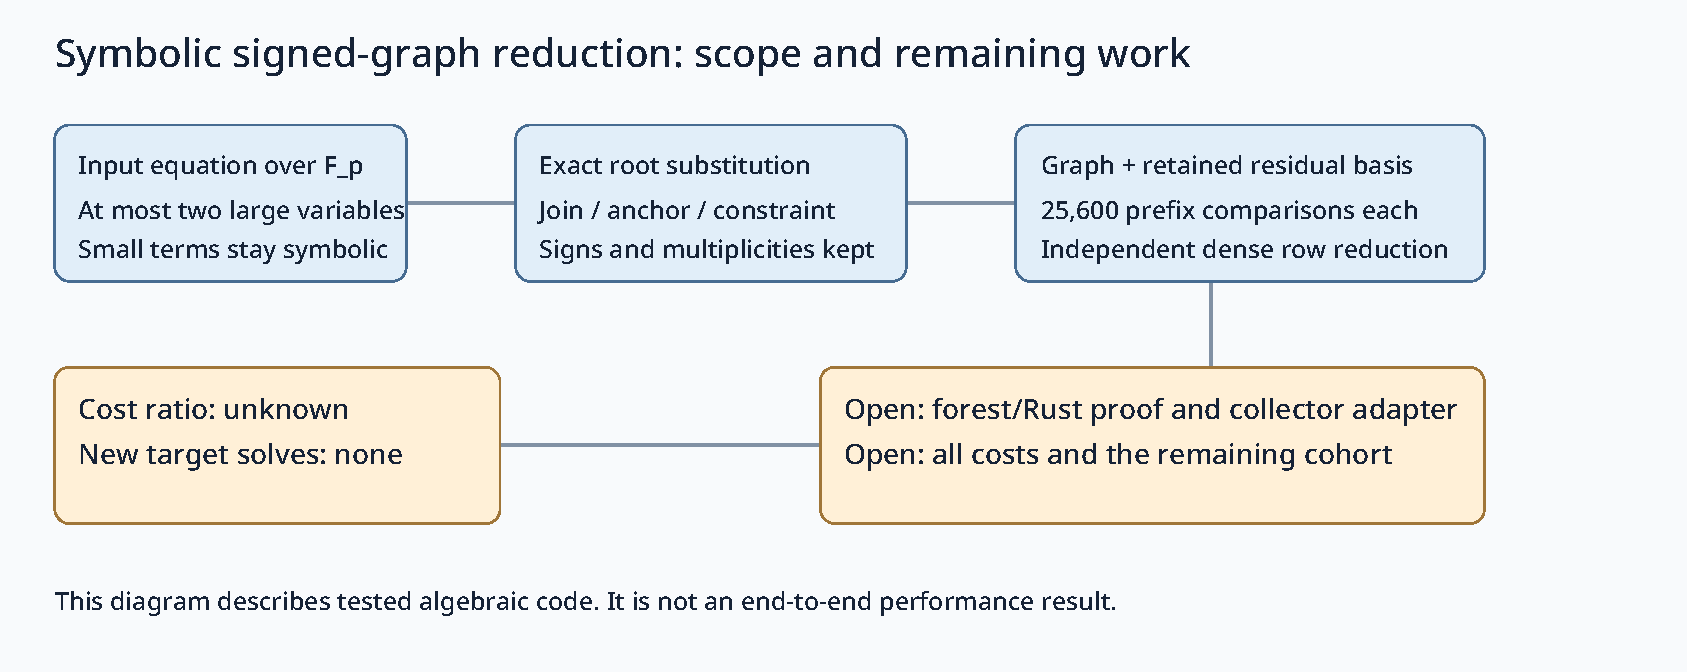
\includegraphics[width=\linewidth]{reduction.pdf}\end{center}
\end{document}
